% Provenance (never printed): cycle 4 SVT/physique, "La planete Terre,
% l'environnement": uneven heating of the Earth, movements of the
% atmosphere, the global circulation and the climate zones; see
% sources/book1/PROVENANCE.md. Book 1, grade 8, chapter 2.
% Vocabulary guard: owns convection cell (atmospheric, descriptive), sea
% breeze and land breeze, the global winds, the global circulation. The
% Coriolis effect is told as "the Earth's rotation deflects"; Hadley and
% Ferrel cells and the intertropical convergence zone are named in prose
% only (Book 3 owns them); mantle convection is Book 2's.
\chapter{风与全球环流}\label{ch:g8:winds-global-circulation}

几个世纪以来，从欧洲和非洲港口驶往美洲的帆船，依靠一种稳定的东风，
这种风在\omterm{def:g3:continents-and-oceans:equator}{赤道}两侧吹拂，载着它们横跨大西洋。
世界各地的水手都熟悉这种风，早期与美洲的贸易也全靠它：它就是
\emph{\omterm{def:g8:winds-global-circulation:global-winds}{信风}}。
如今，货船仍借助\omterm{def:g8:winds-global-circulation:global-winds}{信风}及其驱动的洋流，
来缩短航程。
% ledger: nos:trade-winds

\begin{omfigure}
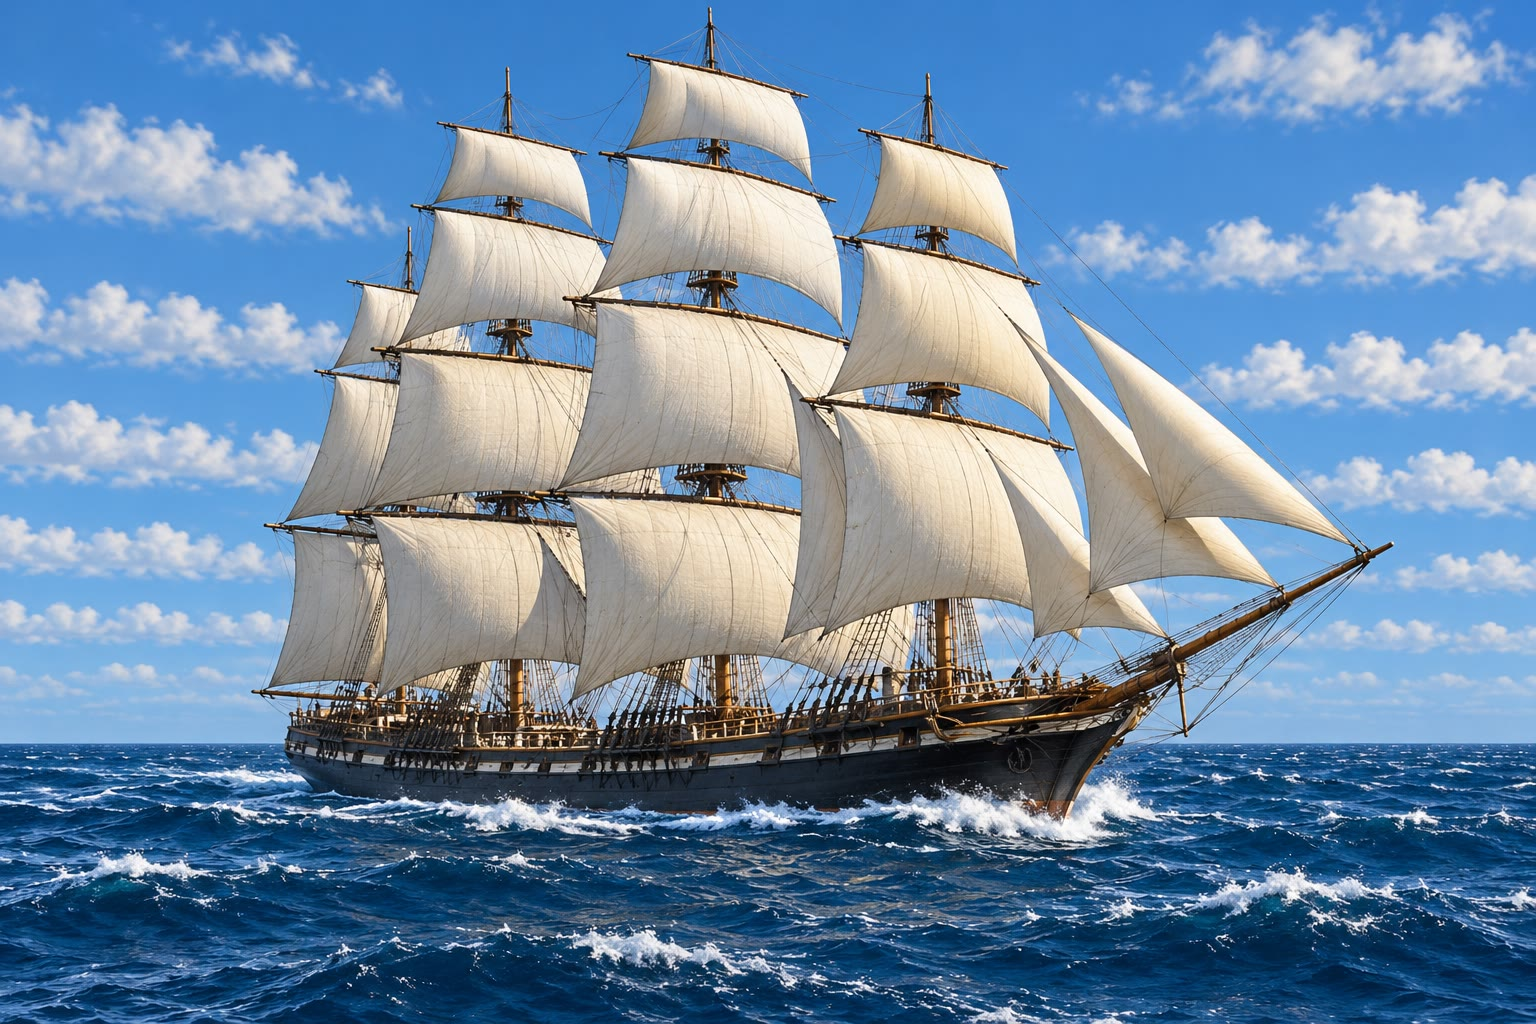
\includegraphics[width=0.62\linewidth]{images/book1/ai/g8-sailing-ship.jpg}

{\small 帆船在开阔的海面上顺着稳定的风航行
（AI 生成的示意图，表现一般场景）。}
\label{fig:g8:winds-global-circulation:ship}
\end{omfigure}

\omterm{def:g8:winds-global-circulation:global-winds}{信风}为何总从东方吹来，而且总在相同的地区？
为什么\omterm{def:g5:weather-and-climate:tropics}{回归线}附近有\omterm{def:g5:weather-and-climate:desert}{沙漠}，\omterm{def:g3:continents-and-oceans:equator}{赤道}附近有\omterm{def:g5:weather-and-climate:rainforest}{雨林}？
答案要从太阳说起。

\begin{recall}
风是运动的空气（见物理分册）。空气压在它接触的一切物体上，
且压强随高度增加而减小，
（\cref{ch:g8:the-atmosphere}）。\omterm{def:g1:watching-the-weather:weather}{天气}发生在\omterm{def:g8:the-atmosphere:layers}{对流层}中，
\omterm{def:g8:the-atmosphere:layers}{对流层}是大气的最底层。地球上有若干\omterm{def:g5:weather-and-climate:climate-zone}{气候带}：\omterm{def:g3:continents-and-oceans:equator}{赤道}附近炎热潮湿，多\omterm{def:g5:weather-and-climate:rainforest}{雨林}；
\omterm{def:g5:weather-and-climate:tropics}{回归线}附近炎热干燥，多\omterm{def:g5:weather-and-climate:desert}{沙漠}；
向两极依次为温带和寒带，
（\cref{ch:g5:weather-and-climate}）。
\end{recall}

\section{太阳对地球的加热不均匀}

在春分或秋分这天的正午，太阳直射\omterm{def:g3:continents-and-oceans:equator}{赤道}。
此处光线很陡，照射在较小的一片地面上。
在\omterm{def:g3:continents-and-oceans:equator}{赤道}以北或以南，同样的光线斜射，
铺展在更大的面积上，每平方米接收的能量较少。
在\omterm{def:g6:latitude-longitude:latitude}{纬度} \ang{60} 处，同一束光覆盖的地面是\omterm{def:g3:continents-and-oceans:equator}{赤道}处的两倍，
因此每平方米接收的能量只有一半。
% ledger: (geometry: figdata/grade-8/sunlight_spread.py, spread = 1/cos(latitude))

\begin{omfigure}
\begin{tikzpicture}[font=\footnotesize]
  \def\R{2.6}\def\w{0.2}
  \fill[blue!10] (0,0) circle (\R);
  \draw (0,0) circle (\R);
  \draw[black!50] (-\R,0) -- (\R,0);
  \draw[black!40, dashed] (0,0) -- (60:\R);
  \draw[black!40] (0,0) ++(0:0.7) arc (0:60:0.7);
  \node at (25:0.95) {\ang{60}};
  \node[anchor=east, black!60] at (-\R-0.05,0) {赤道};
  % beam at the equator: rays between y = -w and y = w
  \foreach \y in {-0.2,-0.1,0,0.1,0.2} {
    \pgfmathsetmacro{\x}{sqrt(\R*\R-\y*\y)}
    \draw[orange!80!black, -{Stealth[length=1.6mm]}] (6.2,\y) -- (\x+0.03,\y);}
  \draw[omThm, line width=2.2pt] ({sqrt(\R*\R-0.35*0.35)},-0.35) arc ({asin(-\w/\R)}:{asin(\w/\R)}:\R);
  % beam near 60 degrees: rays between y = R sin 60 - w and + w
  \pgfmathsetmacro{\yc}{\R*sin(60)}
  \foreach \d in {-0.2,-0.1,0,0.1,0.2} {
    \pgfmathsetmacro{\y}{\yc+\d}
    \pgfmathsetmacro{\x}{sqrt(\R*\R-\y*\y)}
    \draw[orange!80!black, -{Stealth[length=1.6mm]}] (6.2,\y) -- (\x+0.03,\y);}
  \draw[omThm, line width=2.2pt] ({sqrt(\R*\R-(\yc-\w)^2)},\yc-\w) arc ({asin((\yc-\w)/\R)}:{asin((\yc+\w)/\R)}:\R);
  \node[anchor=west, align=left] at (6.3,0) {同一束光 \\照在较小的一片地面上};
  \node[anchor=west, align=left] at (6.3,\yc) {同一束光铺展在 \\两倍大的地面上};
\end{tikzpicture}

{\small 春分或秋分正午的两束相同的阳光。在
\omterm{def:g3:continents-and-oceans:equator}{赤道}处，光束垂直照射在较小的一片地面上（粗线）；在
\omterm{def:g6:latitude-longitude:latitude}{纬度} \ang{60} 处，光束斜射，覆盖的地面是原来的两倍。}
% ledger: (geometry: figdata/grade-8/sunlight_spread.py)
\label{fig:g8:winds-global-circulation:beams}
\end{omfigure}

\begin{center}\small
\begin{tabular}{|l|c|c|c|c|c|}
\hline
\omterm{def:g6:latitude-longitude:latitude}{纬度} & \ang{0} & \ang{30} & \ang{45} & \ang{60} & \ang{75} \\
\hline
同一束光覆盖的地面 & 1 & 1.15 & 1.41 & 2 & 3.86 \\
\hline
每平方米接收的能量（占\omterm{def:g3:continents-and-oceans:equator}{赤道}处的\%） & 100 & 87 & 71 & 50 & 26 \\
\hline
\end{tabular}
\end{center}
% ledger: (figdata/grade-8/sunlight_spread.py main table)

地球绕太阳公转时，地轴的倾斜使直射点
在两条\omterm{def:g5:weather-and-climate:tropics}{回归线}之间移动，从而形成季节（见物理分册）；
但全年来看，\omterm{def:g3:continents-and-oceans:equator}{赤道}附近获得的能量远多于两极附近。
这种不均匀的加热是风的主要驱动：大气
把暖空气输送向两极，
把冷空气输送向\omterm{def:g3:continents-and-oceans:equator}{赤道}。
% ledger: mo:global-circ

\section{上升与下沉的空气}

暖空气比冷空气轻，于是上升，周围较冷的空气
流入以补充其位置。空气上升处，对地面的压力较小，气压低；
空气下沉处，压力较大，气压高。
在近地面，风由高压吹向低压。
空气上升、冷却、下沉、再回流，
如此循环往复，形成一个环流。
% ledger: jetstream:sea-breeze, mo:three-cells

\begin{definition}[对流环流]\label{def:g8:winds-global-circulation:convection-cell}
大气中的\emph{对流环流}\index{对流环流}是一种空气的运动环路：
从下方受热的空气上升，在高处向四周扩散，
在别处冷却下沉，并沿地面流回原先上升的地方。
上升空气之下气压低；
下沉空气之下气压高。
\end{definition}
% ledger: jetstream:sea-breeze, mo:three-cells

\begin{inthelab}[暖空气上升]
在室内，从一张薄纸上剪出一个螺旋形，形如苹果皮，
用细线在中心处将其挂起。冬季把它悬在暖气片上方较高处
（切勿放在火焰或蜡烛上方），它会慢慢开始转动。
暖气片加热的空气上升，推动螺旋形纸片。
把它靠近冷窗户：它会向相反方向转动，还是完全不动？
\end{inthelab}

晴天在海边，可以感受到最小的\omterm{def:g8:winds-global-circulation:convection-cell}{对流环流}。
陆地与\omterm{def:g2:water-on-earth:ocean}{海洋}接受的阳光相同，但阳光无法深入地下，
而\omterm{def:g2:water-on-earth:ocean}{海洋}能将热量分散到较厚的水层中。
因此白天陆地升温远比\omterm{def:g2:water-on-earth:ocean}{海洋}快，
夜间降温也远比\omterm{def:g2:water-on-earth:ocean}{海洋}快。
% ledger: jetstream:sea-breeze

\begin{omfigure}
\begin{tikzpicture}[font=\footnotesize, >={Stealth[length=2mm]}]
  \foreach \px/\title/\dir in {0/{白天：海风}/1, 8.3/{夜间：陆风}/-1} {
    \begin{scope}[xshift=\px cm]
      \fill[omSea] (0,0) rectangle (3.5,0.45);
      \fill[omLithAlluv] (3.5,0) -- (3.5,0.45) -- (7,0.75) -- (7,0) -- cycle;
      \draw (0,0.45) -- (3.5,0.45) -- (7,0.75);
      \node[anchor=south] at (3.5,3.25) {\textbf{\title}};
      \node at (1.75,0.22) {海};
      \node at (5.6,0.3) {陆地};
    \end{scope}}
  % day loop: surface sea -> land, rise over land, return aloft, sink over sea
  \draw[->, omDef, line width=1.1pt] (1.2,0.8) -- (5.2,0.95);
  \draw[->, omThm, line width=1.1pt] (5.8,1.1) -- (5.8,2.4);
  \draw[->, black!60, line width=1.1pt] (5.2,2.75) -- (1.2,2.75);
  \draw[->, omDef, line width=1.1pt] (0.6,2.4) -- (0.6,1.1);
  \node[omDef] at (3.2,1.25) {海风};
  \node at (0.6,0.75) {\textbf{H}};
  \node at (5.8,0.95) {\textbf{L}};
  \fill[yellow!80!orange] (6.6,2.7) circle (0.25);
  \node[anchor=north, align=center] at (1.75,-0.1) {较冷的海洋};
  \node[anchor=north, align=center] at (5.3,-0.1) {较暖的陆地};
  % night loop: surface land -> sea, rise over sea, return aloft, sink over land
  \begin{scope}[xshift=8.3cm]
    \draw[->, omDef, line width=1.1pt] (5.2,1.0) -- (1.2,0.8);
    \draw[->, omThm, line width=1.1pt] (0.6,1.1) -- (0.6,2.4);
    \draw[->, black!60, line width=1.1pt] (1.2,2.75) -- (5.2,2.75);
    \draw[->, omDef, line width=1.1pt] (5.8,2.4) -- (5.8,1.15);
    \node[omDef] at (3.2,1.3) {陆风};
    \node at (0.6,0.75) {\textbf{L}};
    \node at (5.8,1.0) {\textbf{H}};
    \fill[black!25] (6.6,2.7) circle (0.25); \fill[white] (6.72,2.78) circle (0.21);
    \node[anchor=north, align=center] at (1.75,-0.1) {较暖的海洋};
    \node[anchor=north, align=center] at (5.3,-0.1) {较冷的陆地};
  \end{scope}
\end{tikzpicture}

{\small \omterm{def:g8:winds-global-circulation:breezes}{海风}与\omterm{def:g8:winds-global-circulation:breezes}{陆风}：两个转向相反的小型\omterm{def:g8:winds-global-circulation:convection-cell}{对流环流}。
红色箭头：上升的暖空气；H 与 L：近地面的高压与低压。
白天，环流可上升至约 1000 至
\qty{1500}{m} 高处。}
% ledger: jetstream:sea-breeze
\label{fig:g8:winds-global-circulation:breezes}
\end{omfigure}

\begin{definition}[海风与陆风]\label{def:g8:winds-global-circulation:breezes}
\emph{海风}\index{海风}是白天从\omterm{def:g2:water-on-earth:ocean}{海洋}吹向
陆地的风，此时陆地比\omterm{def:g2:water-on-earth:ocean}{海洋}暖。\emph{陆风}\index{陆风}
是夜间从陆地吹向\omterm{def:g2:water-on-earth:ocean}{海洋}的风，
此时陆地已比\omterm{def:g2:water-on-earth:ocean}{海洋}冷。
\end{definition}
% ledger: jetstream:sea-breeze

\begin{omfigure}
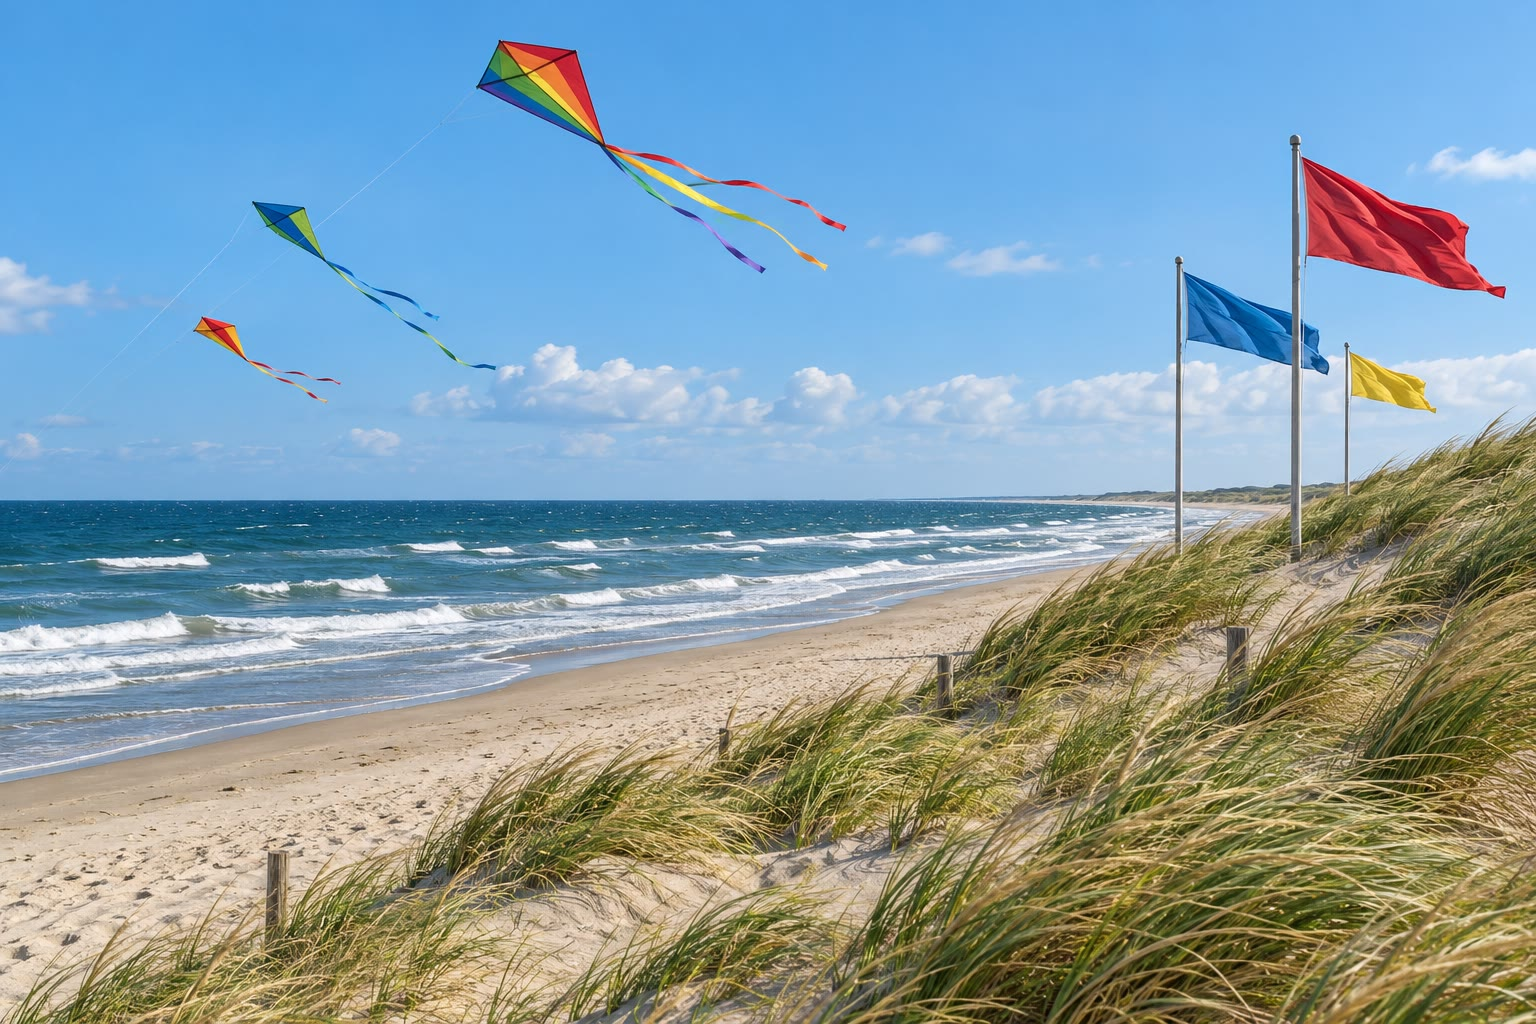
\includegraphics[width=0.55\linewidth]{images/book1/ai/g8-beach-kites.jpg}

{\small 海滩上，风筝在午后的风中飘扬（AI 生成的
通用场景插图）。}
\label{fig:g8:winds-global-circulation:kites}
\end{omfigure}

\section{全球性风系}

同样的过程也发生在整个地球的尺度上。
\omterm{def:g3:continents-and-oceans:equator}{赤道}附近，强烈受热的空气上升，
在高处向两极扩散，并在约 \ang{30} \omterm{def:g6:latitude-longitude:latitude}{纬度}处再次下沉。多年平均来看，
每个\omterm{def:g3:continents-and-oceans:equator}{半球}的\omterm{def:g8:the-atmosphere:layers}{对流层}分为三个大型\omterm{def:g8:winds-global-circulation:convection-cell}{对流环流}：
一个从\omterm{def:g3:continents-and-oceans:equator}{赤道}到约 \ang{30}，一个从约 \ang{30} 到
约 \ang{60}，一个从约 \ang{60} 到极点。
气象学家称之为哈得来环流圈、费雷尔环流圈与极地环流圈。
它们的边界随季节移动，中间的环流圈则是许多经过的\omterm{def:g5:natural-hazards:storm}{风暴}的粗略平均。
% ledger: mo:three-cells, mo:global-circ, nos:doldrums

若地球不自转，近地面的风将直接由高压吹向低压。
由于地球自转，运动的空气会发生偏转：
\omterm{def:g3:continents-and-oceans:equator}{北半球}向右偏，\omterm{def:g3:continents-and-oceans:equator}{南半球}向左偏。
因此回流至\omterm{def:g3:continents-and-oceans:equator}{赤道}的空气并非来自北方，
而是在\omterm{def:g3:continents-and-oceans:equator}{北半球}来自东北方，
在\omterm{def:g3:continents-and-oceans:equator}{南半球}来自东南方。
% ledger: mo:global-circ, nos:trade-winds

\begin{definition}[全球性风系]\label{def:g8:winds-global-circulation:global-winds}
各\omterm{def:g6:latitude-longitude:latitude}{纬度}带中最常吹的近地面风如下：
\begin{itemize}
  \item \emph{信风}\index{信风}，位于\omterm{def:g3:continents-and-oceans:equator}{赤道}与
        约 \ang{30} 之间，\omterm{def:g3:continents-and-oceans:equator}{北半球}吹东北风，
        \omterm{def:g3:continents-and-oceans:equator}{南半球}吹东南风；
  \item \emph{西风带}\index{西风带}，位于约 \ang{30}
        与约 \ang{60} 之间，吹西风（\omterm{def:g3:continents-and-oceans:equator}{北半球}为西南风，
        \omterm{def:g3:continents-and-oceans:equator}{南半球}为西北风）；
  \item \emph{极地东风带}\index{极地东风带}，位于约
        \ang{60} 与极点之间，吹东风。
\end{itemize}
\end{definition}
% ledger: nos:trade-winds, mo:three-cells, mo:global-circ

\begin{omfigure}
\begin{tikzpicture}[font=\scriptsize, >={Stealth[length=1.8mm]}]
  \def\R{3}
  \fill[blue!8] (0,0) circle (\R);
  \draw (0,0) circle (\R);
  \draw[black!45] (-\R,0) -- (\R,0);
  \foreach \l in {-60,-30,30,60} {
    \pgfmathsetmacro{\y}{\R*sin(\l)}
    \pgfmathsetmacro{\x}{\R*cos(\l)}
    \draw[black!45, dashed] (-\x,\y) -- (\x,\y);}
  % surface winds: NE trades, SW westerlies, NE polar easterlies (north); mirrored south
  \foreach \x in {-1.8,-0.6,0.6,1.8} {
    \draw[->, omThm, line width=0.9pt] (\x+0.35,0.95) -- (\x-0.35,0.55);
    \draw[->, omThm, line width=0.9pt] (\x+0.35,-0.95) -- (\x-0.35,-0.55);}
  \foreach \x in {-1.2,0,1.2} {
    \draw[->, omDef, line width=0.9pt] (\x-0.35,1.7) -- (\x+0.35,2.02);
    \draw[->, omDef, line width=0.9pt] (\x-0.35,-1.7) -- (\x+0.35,-2.02);}
  \foreach \x in {-0.4,0.4} {
    \draw[->, omMeth, line width=0.9pt] (\x+0.25,2.85) -- (\x-0.25,2.65);
    \draw[->, omMeth, line width=0.9pt] (\x+0.25,-2.85) -- (\x-0.25,-2.65);}
  \node[fill=blue!8, inner sep=1pt] at (0,1.2) {东北信风};
  \node[fill=blue!8, inner sep=1pt] at (0,-1.2) {东南信风};
  \node[fill=blue!8, inner sep=1pt] at (0,2.3) {西风带};
  \node[fill=blue!8, inner sep=1pt] at (0,-2.3) {西风带};
  \node[anchor=south] at (0,\R+0.05) {极地东风带};
  \node[anchor=north] at (0,-\R-0.05) {极地东风带};
  % pressure belts on the left
  \foreach \l/\t in {90/{高压：空气下沉}, 60/{低压：空气上升}, 30/{高压：空气下沉，干燥，多沙漠}, 0/{低压：空气上升，多云，降雨}, -30/{高压：空气下沉，干燥，多沙漠}, -60/{低压：空气上升}, -90/{高压：空气下沉}} {
    \pgfmathsetmacro{\y}{\R*sin(\l)}
    \pgfmathsetmacro{\x}{\R*cos(\l)}
    \draw[black!40] (-\x-0.05,\y) -- (-3.35,\y);
    \node[anchor=east] at (-3.4,\y) {\t};}
  \foreach \l/\t in {60/{北纬 \ang{60}}, 30/{北纬 \ang{30}}, 0/{赤道}, -30/{南纬 \ang{30}}, -60/{南纬 \ang{60}}} {
    \pgfmathsetmacro{\y}{\R*sin(\l)}
    \pgfmathsetmacro{\x}{\R*cos(\l)}
    \node[anchor=west, black!60] at (\x+0.05,\y) {\t};}
  % side view of the cells (height to the right), same latitude scale
  \begin{scope}[xshift=5.2cm]
    \draw[->] (0,-\R) -- (0,\R+0.3);
    \draw (0,-\R) -- (1.8,-\R);
    \node[anchor=north, align=center] at (0.9,-\R-0.05) {对流层中 \\高度 $\rightarrow$};
    \foreach \lo/\hi/\cw in {0/30/0, 30/60/1, 60/90/0, -30/0/1, -60/-30/0, -90/-60/1} {
      \pgfmathsetmacro{\ya}{\R*sin(\lo)}
      \pgfmathsetmacro{\yb}{\R*sin(\hi)}
      \pgfmathsetmacro{\yc}{(\ya+\yb)/2}
      \pgfmathsetmacro{\bb}{max(0.09,(\yb-\ya)/2-0.06)}
      \ifnum\cw=0
        \draw[black!70, line width=0.7pt, postaction={decorate}, decoration={markings,
          mark=at position 0.125 with {\arrow{Stealth[length=1.6mm]}}, mark=at position 0.375 with {\arrow{Stealth[length=1.6mm]}},
          mark=at position 0.625 with {\arrow{Stealth[length=1.6mm]}}, mark=at position 0.875 with {\arrow{Stealth[length=1.6mm]}}}]
          (0.9,\yc) ++(0.75,0) arc (0:360:0.75 and \bb);
      \else
        \draw[black!70, line width=0.7pt, postaction={decorate}, decoration={markings,
          mark=at position 0.125 with {\arrow{Stealth[length=1.6mm]}}, mark=at position 0.375 with {\arrow{Stealth[length=1.6mm]}},
          mark=at position 0.625 with {\arrow{Stealth[length=1.6mm]}}, mark=at position 0.875 with {\arrow{Stealth[length=1.6mm]}}}]
          (0.9,\yc) ++(0.75,0) arc (360:0:0.75 and \bb);
      \fi}
  \end{scope}
\end{tikzpicture}

{\small 大气环流示意图（简化）。左：地面高压带（H）与低压带
（L）的分布。\omterm{def:g3:continents-and-oceans:globe}{地球仪}上：经地球自转偏转后的
地面风。右：每个\omterm{def:g3:continents-and-oceans:equator}{半球}的三个\omterm{def:g8:winds-global-circulation:convection-cell}{对流环流}，
从侧面看，\omterm{def:g6:latitude-longitude:latitude}{纬度}与左图相同（极地环流
画得很细，因为极地带在\omterm{def:g3:continents-and-oceans:globe}{地球仪}上较窄
）。}
% ledger: mo:three-cells, mo:global-circ, nos:trade-winds, nos:doldrums
\label{fig:g8:winds-global-circulation:cells}
\end{omfigure}

\begin{method}[求某纬度处的全球风]\label{met:g8:winds-global-circulation:wind}
\begin{enumerate}
  \item 找出所在的带：从\omterm{def:g3:continents-and-oceans:equator}{赤道}到约 \ang{30}，从 \ang{30}
        到 \ang{60}，或从 \ang{60} 到极点。
  \item 找出该带地面空气的流动方向：
        在第一带和最后一带流向\omterm{def:g3:continents-and-oceans:equator}{赤道}，在
        中间一带流向极地。
  \item 将该流动偏转：\omterm{def:g3:continents-and-oceans:equator}{北半球}向右偏，\omterm{def:g3:continents-and-oceans:equator}{南半球}
        向左偏。
  \item 说明风的来向：风以其
        \emph{来自}的方向命名。
\end{enumerate}
\end{method}

\begin{example}[南纬 \ang{40} 处的风]\label{ex:g8:winds-global-circulation:40s}
在南纬 \ang{40}，位于中间一带，即 \ang{30} 与 \ang{60} 之间。
该处地面空气流向极地，即流向南方。在\omterm{def:g3:continents-and-oceans:equator}{南半球}，它向左偏转：
对于向南运动的空气，左侧是东方，因此空气最终朝
东南方向运动，
所以它来自西北方，属于
\omterm{def:g8:winds-global-circulation:global-winds}{西风带}之一，由西北方吹来。
\end{example}
% ledger: mo:three-cells, mo:global-circ

\omterm{def:g3:continents-and-oceans:equator}{赤道}附近，两个\omterm{def:g3:continents-and-oceans:equator}{半球}的\omterm{def:g8:winds-global-circulation:global-winds}{信风}在此汇合，风力减弱，
水手们称这一平静的带为
\emph{无风带}。这里温暖潮湿的空气上升，冷却后
形成持续性阵雨与雷暴。在约 \ang{30} 附近，下沉气流之下，
风力较弱，降雨稀少。
% ledger: nos:doldrums

\begin{definition}[大气的全球环流]\label{def:g8:winds-global-circulation:circulation}
大气的\emph{全球环流}\index{全球环流}是指空气在全球范围内的大尺度运动，
对许多年的风进行平均后可以看出。它将热量
从\omterm{def:g3:continents-and-oceans:equator}{赤道}输送到极地，并将水汽从一个
\omterm{def:g6:latitude-longitude:latitude}{纬度}带输送到另一个
\omterm{def:g6:latitude-longitude:latitude}{纬度}带。
\end{definition}
% ledger: mo:global-circ

\section{全球环流与气候带}

\omterm{def:g8:winds-global-circulation:circulation}{全球环流}很大程度上解释了\omterm{def:g5:weather-and-climate:climate-chart}{气候图}的分布。在\omterm{def:g3:continents-and-oceans:equator}{赤道}附近，空气上升时降温，
其中的水汽凝结成云：降雨频繁，\omterm{def:g5:weather-and-climate:rainforest}{雨林}茂盛。
在北纬和南纬 \ang{30} 附近，空气下沉，升温，
\omterm{def:g4:clouds-rain-snow:cloud}{云层}消散，降雨稀少：大片炎热的\omterm{def:g5:weather-and-climate:desert}{沙漠}，
如撒哈拉\omterm{def:g5:weather-and-climate:desert}{沙漠}，就位于这些\omterm{def:g6:latitude-longitude:latitude}{纬度}带上。在中\omterm{def:g6:latitude-longitude:latitude}{纬度}地区，
\omterm{def:g8:winds-global-circulation:global-winds}{西风带}带来一个接一个的\omterm{def:g5:natural-hazards:storm}{风暴}，
四季都有降雨。
% ledger: nos:doldrums, mo:three-cells, mo:global-circ

\begin{omfigure}
\begin{minipage}[c]{0.42\linewidth}\centering
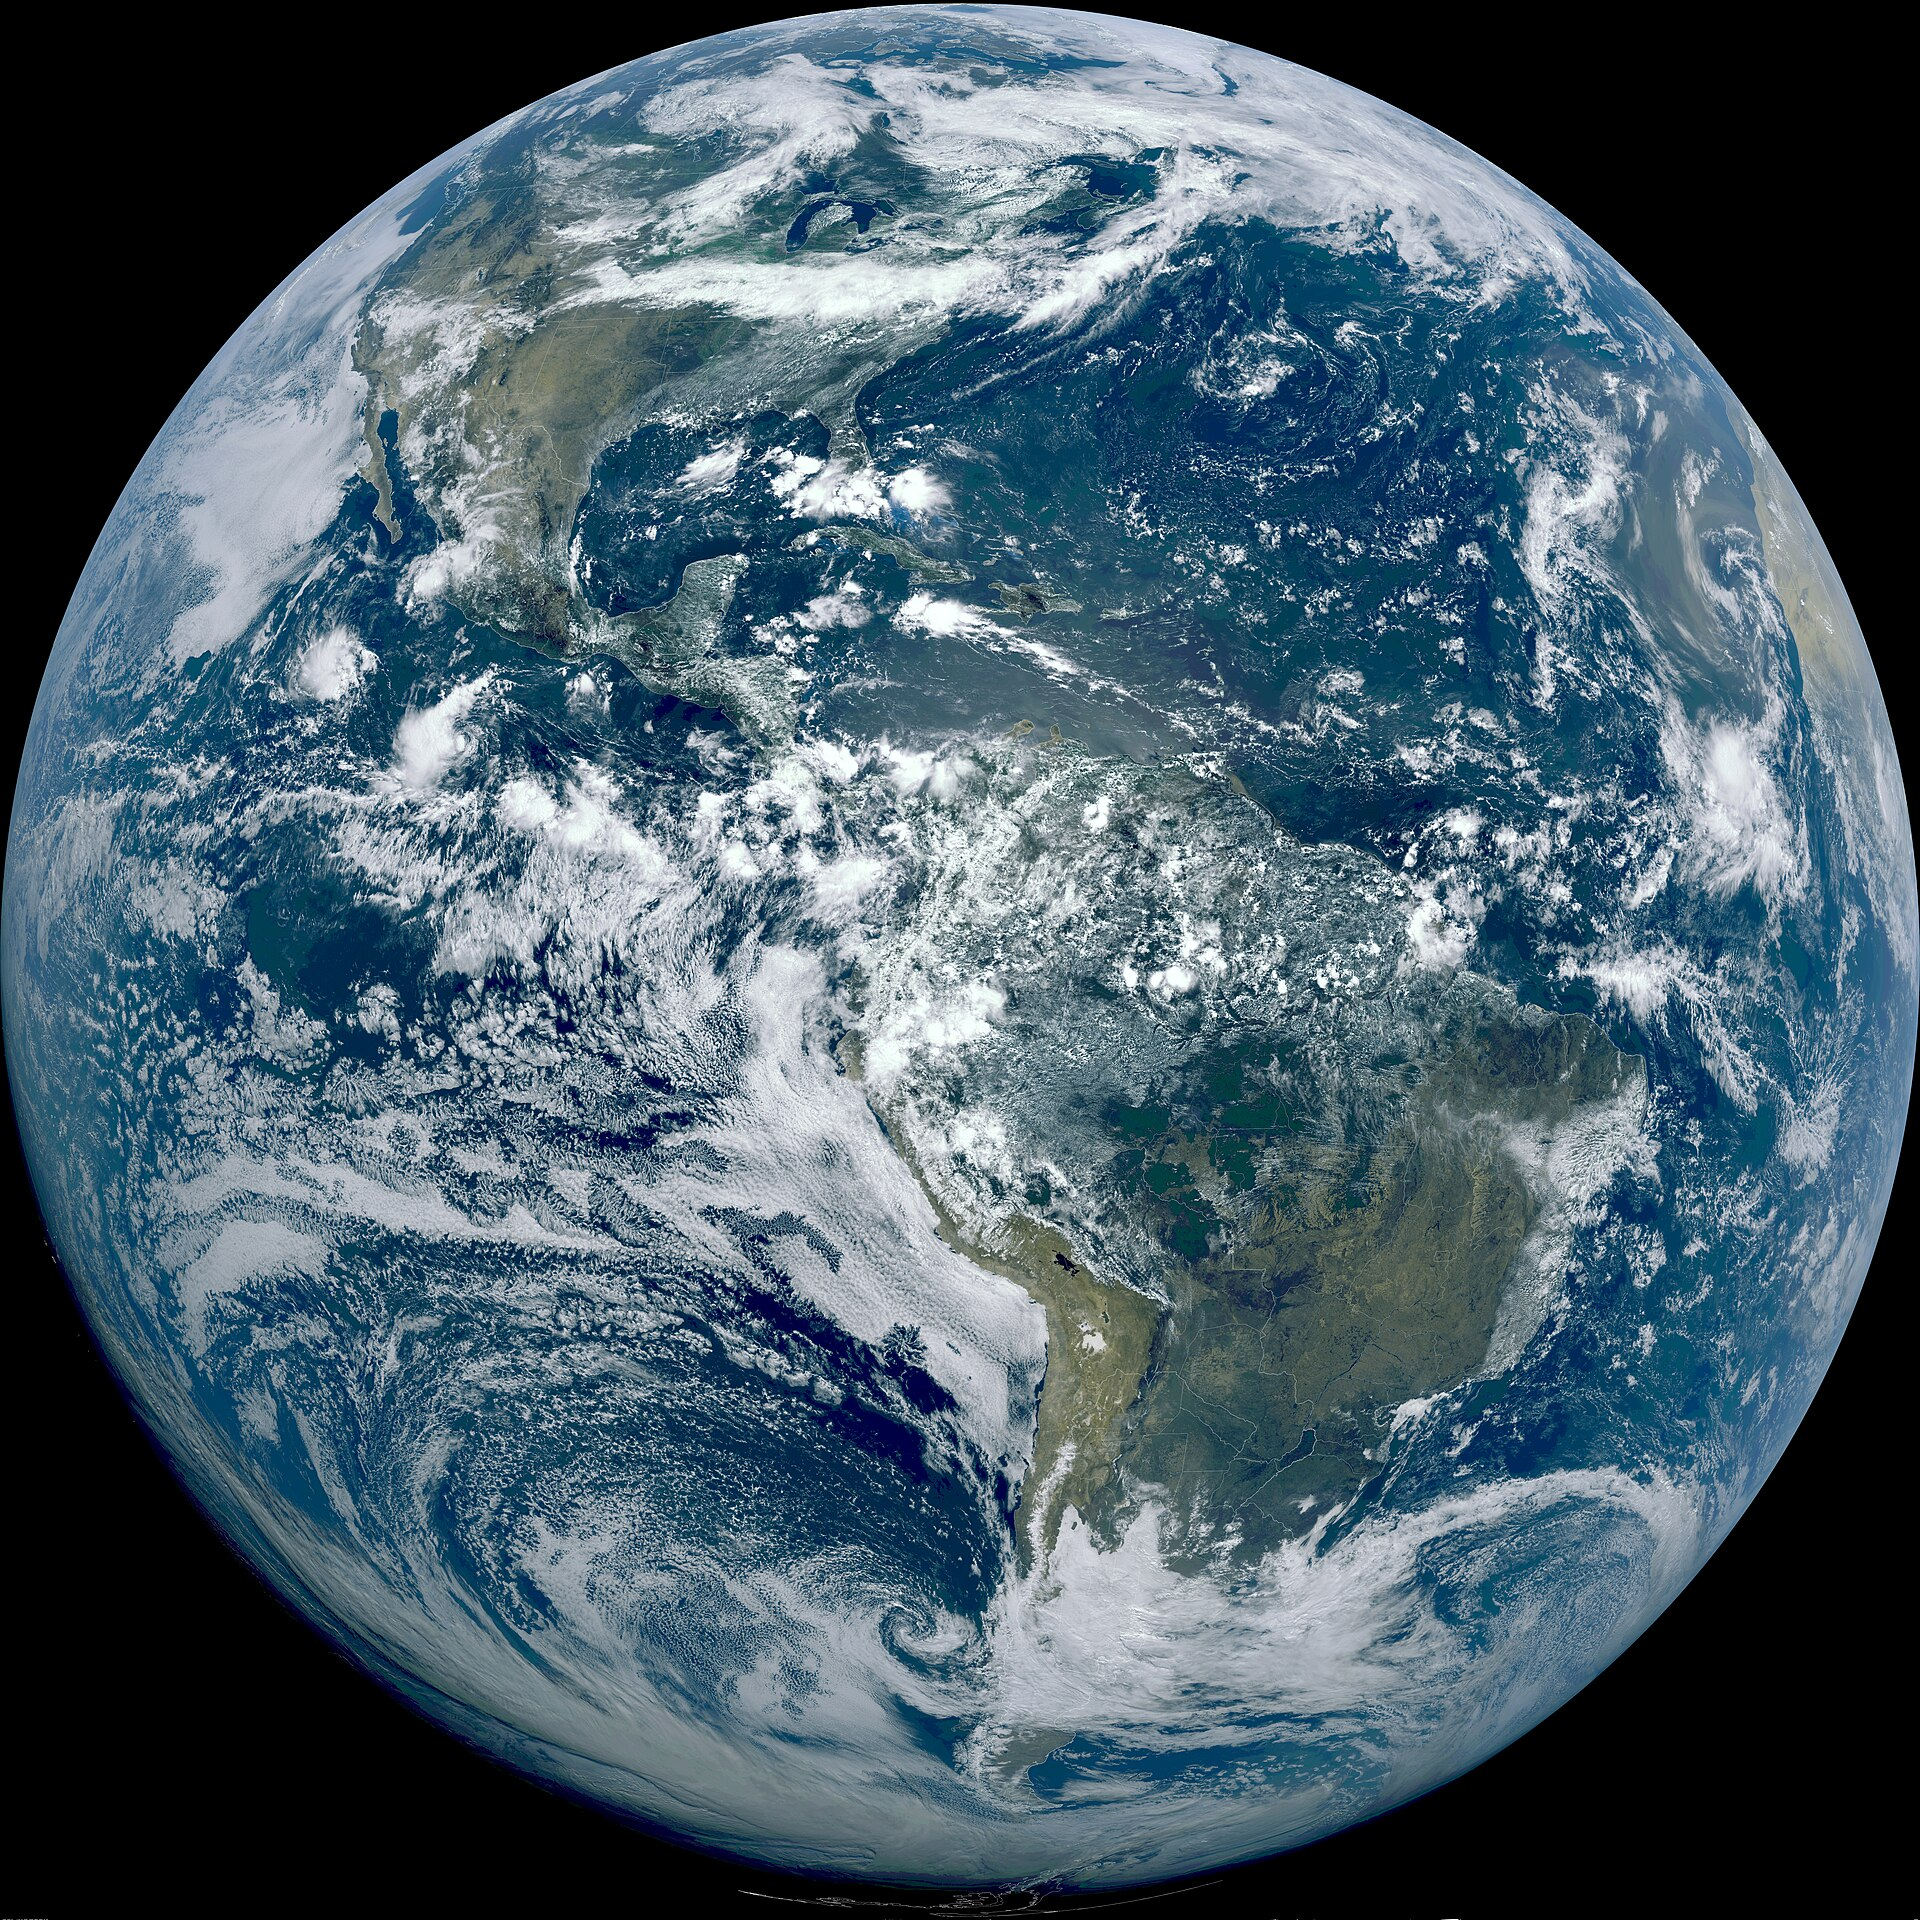
\includegraphics[width=\linewidth]{images/book1/g8-goes-full-disk.jpg}
\end{minipage}\hfill
\begin{minipage}[c]{0.54\linewidth}\raggedright
{\small 2022 年 7 月 26 日，GOES-16 气象卫星从\omterm{def:g3:continents-and-oceans:equator}{赤道}上空拍摄的美洲图像，
热带地区和亚马孙\omterm{def:g5:weather-and-climate:rainforest}{雨林}上空形成了许多云，那里温暖潮湿的空气正在上升；
更南的地方正值\omterm{def:g3:continents-and-oceans:equator}{南半球}冬季，\omterm{def:g8:winds-global-circulation:global-winds}{西风带}的\omterm{def:g5:natural-hazards:storm}{风暴}
在海面上盘旋。
图片来源：NOAA（公有领域，经维基共享资源）。}
\end{minipage}
% ledger: commons:goes16, nos:doldrums
\label{fig:g8:winds-global-circulation:goes}
\end{omfigure}

\begin{example}[四个城镇，四条纬度带]\label{ex:g8:winds-global-circulation:four-towns}
\cref{ch:g5:weather-and-climate} 中\omterm{def:g5:weather-and-climate:climate-chart}{气候图}里的四个城镇
都位于\omterm{def:g3:continents-and-oceans:equator}{北半球}，\omterm{def:g6:latitude-longitude:latitude}{纬度}差别很大。
它们每年的降雨和降雪符合\omterm{def:g8:winds-global-circulation:circulation}{全球环流}的\omterm{def:g6:latitude-longitude:latitude}{纬度}带分布（见下图）。
希洛位于北纬 \ang{20}，是\omterm{def:g2:water-on-earth:ocean}{海洋}中一座岛屿，
处于\omterm{def:g8:winds-global-circulation:global-winds}{信风}带，\omterm{def:g8:winds-global-circulation:global-winds}{信风}在这里携带大量水汽，每年约
降 \qty{3000}{mm}。菲尼克斯位于北纬 \ang{33}，接近 \ang{30}，
处于下沉气流之下：年\omterm{def:g4:clouds-rain-snow:precipitation}{降水}量不足 \qty{200}{mm}。西雅图位于
北纬 \ang{47}，处于\omterm{def:g8:winds-global-circulation:global-winds}{西风带}，\omterm{def:g8:winds-global-circulation:global-winds}{西风带}的\omterm{def:g5:natural-hazards:storm}{风暴}
每年带来约 \qty{1000}{mm} \omterm{def:g4:clouds-rain-snow:precipitation}{降水}，大部分集中在秋季至次年春季。乌特恰维克位于
北纬 \ang{71}，处于近极地下沉的冷空气之下，
年\omterm{def:g4:clouds-rain-snow:precipitation}{降水}量不足 \qty{150}{mm}，是一座寒冷的\omterm{def:g5:weather-and-climate:desert}{沙漠}。
% ledger: data:b1-noaa-normals (totals from figdata/grade-5/climate_charts.py, re-read in figdata/grade-8/rain_by_belt.py), mo:three-cells, nos:doldrums
\end{example}

\begin{omfigure}
\begin{tikzpicture}
\begin{axis}[xbar, width=0.82\linewidth, height=6.4cm, bar width=9pt,
  xmin=0, xmax=3600, ymin=0, ymax=90, ytick={0,30,60,90},
  yticklabels={$0^\circ$, 北纬 $30^\circ$, 北纬 $60^\circ$, 北纬 $90^\circ$},
  xlabel={年降雨和降雪量（mm）}, ylabel={纬度},
  axis x line=bottom, axis y line=left, axis line style={-},
  tick label style={font=\scriptsize}, label style={font=\small},
  xtick={0,1000,2000,3000}, scaled x ticks=false, clip=false,
  point meta=explicit symbolic, nodes near coords,
  nodes near coords style={font=\scriptsize, anchor=west}]
  \draw[black!35, dashed] (axis cs:0,30) -- (axis cs:3600,30);
  \draw[black!35, dashed] (axis cs:0,60) -- (axis cs:3600,60);
  \node[font=\scriptsize, black!60, anchor=south east] at (axis cs:3600,1) {上升气流：降雨};
  \node[font=\scriptsize, black!60, anchor=south east] at (axis cs:3600,30) {下沉气流：干燥};
  \node[font=\scriptsize, black!60, anchor=south east] at (axis cs:3600,60) {上升气流：降雨};
  \node[font=\scriptsize, black!60, anchor=north east] at (axis cs:3600,90) {下沉气流：干燥};
  \addplot[fill=blue!35, draw=blue!60!black] table[x=total_mm, y=lat, meta=name] {figdata/out/grade-8-rain_by_belt-stations.dat};
\end{axis}
\end{tikzpicture}

{\small \omterm{def:g5:weather-and-climate:climate-chart}{气候图}中四个城镇 1991--2020 年平均的年降雨和降雪量，
按\omterm{def:g6:latitude-longitude:latitude}{纬度}标在图中。潮湿的城镇位于空气上升处，即\omterm{def:g3:continents-and-oceans:equator}{赤道}附近和 \ang{60} 附近；
干燥的城镇位于空气下沉处，即 \ang{30} 附近和极地附近。
数据来源：NOAA \omterm{def:g5:weather-and-climate:climate}{气候}平均值。}
% ledger: data:b1-noaa-normals, mo:three-cells (figdata/grade-8/rain_by_belt.py)
\end{omfigure}

四个城镇只是四个点：\omterm{def:g4:world-physical-map:range}{山脉}、\omterm{def:g1:landscapes-around-us:water}{海岸}以及冷暖\omterm{def:g2:water-on-earth:ocean}{海洋}，
也会影响一个地方获得的降雨量。\omterm{def:g6:latitude-longitude:latitude}{纬度}带给出的只是\omterm{def:g5:weather-and-climate:climate-chart}{气候图}的大致格局，
并不代表每个城镇的降雨。

\section{练习}

\begin{exercise}[$\star$]\label{exo:g8:winds-global-circulation:1}
指出下列各处最常吹的全球性风：(a) 北纬 \ang{15}；
(b) 南纬 \ang{45}；(c) 北纬 \ang{75}；(d) 南纬 \ang{20}。
每次都说明其风向。
\end{exercise}

\begin{exercise}[$\star$]\label{exo:g8:winds-global-circulation:2}
补全下列句子。(a) 暖空气\dots{}，冷空气\dots{}。
(b) 在上升气流之下，地面气压\dots{}。(c) 在地面，风从\dots{}
气压吹向\dots{}气压。(d) 在\omterm{def:g3:continents-and-oceans:equator}{北半球}，地球自转使运动的空气向\dots{}
偏转。
\end{exercise}

\begin{exercise}[$\star$]\label{exo:g8:winds-global-circulation:3}
判断下列说法是否正确，并改正错误的句子。(a) \omterm{def:g8:winds-global-circulation:breezes}{海风}从陆地吹向\omterm{def:g2:water-on-earth:ocean}{海洋}。
(b) 白天，陆地比\omterm{def:g2:water-on-earth:ocean}{海洋}升温更快。
(c) \omterm{def:g8:winds-global-circulation:global-winds}{信风}从西方吹来。(d) 许多大\omterm{def:g5:weather-and-climate:desert}{沙漠}位于
\omterm{def:g6:latitude-longitude:latitude}{纬度} \ang{30} 附近。
\end{exercise}

\begin{exercise}[$\star$]\label{exo:g8:winds-global-circulation:4}
画一段\omterm{def:g1:landscapes-around-us:water}{海岸}，海在左侧，陆地在右侧。
加上太阳，然后用箭头画出\omterm{def:g8:winds-global-circulation:breezes}{海风}的空气环流。
在地面气压高和低的位置分别标出 H 和 L。
\end{exercise}

\begin{exercise}[$\star\star$]\label{exo:g8:winds-global-circulation:5}
利用本章中的光束表。(a) 在 \ang{45} 处，一束光束覆盖的地面
面积比\omterm{def:g3:continents-and-oceans:equator}{赤道}处大多少？(b) 在 \ang{60} 处，每平方米接收的
能量占\omterm{def:g3:continents-and-oceans:equator}{赤道}能量的百分之几？(c) 在 \ang{75} 处呢？
(d) 用一句话解释为什么极地寒冷。
\end{exercise}

\begin{exercise}[$\star\star$]\label{exo:g8:winds-global-circulation:6}
一艘船沿正南方向航行，先穿过\omterm{def:g3:continents-and-oceans:equator}{北半球}，
再进入\omterm{def:g3:continents-and-oceans:equator}{南半球}。(a) 它依次遇到哪些风，
从北纬 \ang{70} 到南纬 \ang{70}？(b) 它可能在哪里遇到无风和频繁阵雨的\omterm{def:g1:watching-the-weather:weather}{天气}？
(c) 在哪里风力较弱、降雨稀少？
\end{exercise}

\begin{exercise}[$\star\star$]\label{exo:g8:winds-global-circulation:7}
在一处海滩上，下午 3 点时，沙面温度为 \qty{31}{\degreeCelsius}，
海面上空为 \qty{22}{\degreeCelsius}。凌晨 3 点时，
陆地温度为 \qty{17}{\degreeCelsius}，海面上空为 \qty{21}{\degreeCelsius}。
(a) 下午 3 点时哪处较暖？风从哪个方向吹来？
(b) 凌晨 3 点时呢？(c) 陆地温度在两个时刻之间变化了多少度？
海面温度呢？(d) 解释
这种差异。
\end{exercise}

\begin{exercise}[$\star\star$]\label{exo:g8:winds-global-circulation:8}
空气从北纬 \ang{30} 附近的高压带流向
\omterm{def:g3:continents-and-oceans:equator}{赤道}。(a) 若不计地球自转，风将从哪个方向吹来？
(b) 在本\omterm{def:g3:continents-and-oceans:equator}{半球}，自转使其向哪一侧偏转？
(c) 那么风实际从哪个方向吹来？(d) 对从南纬 \ang{30}
流向\omterm{def:g3:continents-and-oceans:equator}{赤道}的空气，回答同样的三个问题。
\end{exercise}

\begin{exercise}[$\star\star$]\label{exo:g8:winds-global-circulation:9}
逐步解释为什么\omterm{def:g3:continents-and-oceans:equator}{赤道}附近降雨如此频繁：
请使用\emph{受热}、\emph{上升}、\emph{冷却}、\emph{云}这几个词。
然后解释为什么北非北纬 \ang{25} 附近有\omterm{def:g5:weather-and-climate:desert}{沙漠}，请使用
\emph{下沉}、\emph{高压}、\emph{干燥}这几个词。
\end{exercise}

\begin{exercise}[$\star\star$]\label{exo:g8:winds-global-circulation:10}
一艘帆船从欧洲西\omterm{def:g1:landscapes-around-us:water}{海岸}北纬 \ang{40} 的港口出发，
前往北纬 \ang{15} 的加勒比海。(a) 在北纬 \ang{40} 处会遇到哪种风？
它会帮助船向西航行吗？(b) 船为什么应
先向南航行？(c) 哪种风把船带向西方，
并位于哪些\omterm{def:g6:latitude-longitude:latitude}{纬度}之间？(d) 返回欧洲时，
船应寻找哪种风，位于哪个\omterm{def:g6:latitude-longitude:latitude}{纬度}？
\end{exercise}

\begin{exercise}[$\star\star\star$]\label{exo:g8:winds-global-circulation:11}
在\omterm{def:g6:latitude-longitude:latitude}{纬度} $L$ 处，春分日正午一束太阳光覆盖的地面，是\omterm{def:g3:continents-and-oceans:equator}{赤道}处同一光束覆盖地面的 $1 \div
\cos L$ 倍（用计算器时，
$\cos 60^\circ = 0.5$）。(a) 验算 \ang{60} 处的值。(b) 利用
$\cos 30^\circ \approx 0.866$，验算 \ang{30} 处的值，结果保留
两位小数。(c) 设一块平放的太阳能板，该日正午在\omterm{def:g3:continents-and-oceans:equator}{赤道}处
每平方米接收 \qty{1000}{W}。同一块板在 \ang{30} 处约能接收多少？
在 \ang{60} 处呢？
\end{exercise}

\begin{exercise}[$\star\star\star$]\label{exo:g8:winds-global-circulation:12}
在每个\omterm{def:g3:continents-and-oceans:equator}{半球}，\omterm{def:g8:winds-global-circulation:circulation}{全球环流}都有三个环流圈。(a) 画出
\omterm{def:g3:continents-and-oceans:equator}{北半球}的侧视图，\omterm{def:g3:continents-and-oceans:equator}{赤道}在底部，
极点在顶部，三个环流圈画成环状，并标出空气
上升和下沉的位置。(b) 在地面标出高压带和低压带。
(c) 添加每个环流圈的地面风，并使其向右偏转。
(d) 利用你的图解释为什么\omterm{def:g8:winds-global-circulation:global-winds}{西风带}
向东北方向吹。
\end{exercise}

\section{问题：乘信风航行}

\begin{problem}[{周末问题——一艘帆船横渡大西洋，从佛得角前往巴巴多斯，
借东北信风航行；航线在地图上量取，
风向在地图上读取，横渡的长度
由此算出}]
\label{pb:g8:winds-global-circulation:1}
% ledger: data:b1-ne-places, earth:Rmean, nos:trade-winds (figdata/grade-8/trade_route.py; the speed is exercise data)
一艘帆船从佛得角群岛的普拉亚出发，
前往巴巴多斯的布里奇敦。\omterm{def:g2:drawing-to-map:map}{地图}上标出了航线和\omterm{def:g8:winds-global-circulation:global-winds}{信风}。

\begin{center}
\begin{tikzpicture}
\begin{axis}[ommap, width=12cm, xmin=-75, xmax=-5, ymin=0, ymax=35, axis equal image,
  xtick={-70,-60,-50,-40,-30,-20,-10}, ytick={0,10,20,30},
  tick label style={font=\scriptsize},
  xlabel={经度（负值为西）}, ylabel={纬度（北）},
  label style={font=\small}, clip mode=individual]
  \addplot[fill=omLithAlluv, draw=black!60, line width=0.3pt] table {figdata/out/grade-8-trade_route-land.dat};
  \addplot[quiver={u=\thisrow{dlon}, v=\thisrow{dlat}}, -{Stealth[length=1.6mm]}, omThm!80, line width=0.7pt]
    table[x=lon, y=lat] {figdata/out/grade-8-trade_route-trades.dat};
  \addplot[omDef, line width=1.3pt, dashed] table {figdata/out/grade-8-trade_route-route.dat};
  \addplot[only marks, mark=*, mark size=2pt, black] table[x=lon, y=lat] {figdata/out/grade-8-trade_route-ports.dat};
  \node[anchor=north, font=\scriptsize\bfseries, fill=white, inner sep=1pt] at (axis cs:-59.6,12.2) {布里奇敦};
  \node[anchor=south, font=\scriptsize\bfseries, fill=white, inner sep=1pt] at (axis cs:-23.5,15.8) {普拉亚};
\end{axis}
\end{tikzpicture}
\end{center}

\noindent\textbf{第一部分——航线。}\par\nopagebreak
\begin{enumerate}[beginpenalty=10000]
  \item 普拉亚位于北纬 \ang{14.9}、西经 \ang{23.5}；布里奇敦位于
        北纬 \ang{13.1}、西经 \ang{59.6}。两地\omterm{def:g6:latitude-longitude:longitude}{经度}相差
        多少度？
  \item 两个港口都靠近北纬 \ang{14}。沿此\omterm{def:g6:latitude-longitude:latitude}{纬线}，\omterm{def:g6:latitude-longitude:longitude}{经度}每
        一度约为 \qty{108}{km}。横渡约多少
        千米？结果取到最接近的百位。
  \item 若在圆形地球上精确测量，最短航线为
        \qty{3896}{km}。第 2 题的答案是否为好的估计？
  \item 两个港口是否位于\omterm{def:g8:winds-global-circulation:global-winds}{信风}带内？请说明理由。
\end{enumerate}

\noindent\textbf{第二部分——风。}\par\nopagebreak
\begin{enumerate}[resume, beginpenalty=10000]
  \item 在这里，\omterm{def:g8:winds-global-circulation:global-winds}{信风}从哪个方向吹来？
  \item 船向西航行。风把船推向前方、后方，
        还是侧方？请结合\omterm{def:g2:drawing-to-map:map}{地图}说明。
  \item 为什么横渡期间\omterm{def:g8:winds-global-circulation:global-winds}{信风}几乎每天
        都从同一方向吹来？
  \item 返回欧洲途中，船长为什么不应
        沿北纬 \ang{14} 向东航行？
\end{enumerate}

\noindent\textbf{第三部分——横渡。}\par\nopagebreak
\begin{enumerate}[resume, beginpenalty=10000]
  \item 设船平均速度为每小时 \qty{7}{km}，
        那么一天 24 小时内能航行多少千米？
  \item 若途中风停了 3 天，
        船将损失多少千米的航程？
  \item 在稳定的\omterm{def:g8:winds-global-circulation:global-winds}{信风}下，船航行
        \qty{3896}{km} 需要多少天？结果保留一位小数。
  \item 精确到整天，横渡持续多长时间？
        是多于还是少于一个月？
\end{enumerate}
\end{problem}
